

%\documentclass[pra,twocolumn,epsfig,rotate,superscriptaddress,showpacs]{revtex4}


% Use only LaTeX2e, calling the article.cls class and 12-point type.

\documentclass[prl,twocolumn,showpacs]{revtex4}
\usepackage{graphicx}
\usepackage{epsfig}
\usepackage{epsf}
\usepackage{amssymb}
\usepackage{amsmath}
\usepackage{amsthm}
\usepackage{multirow}
\usepackage{hyperref}

\newcommand{\bra}[1]{\langle #1|}
\newcommand{\ket}[1]{|#1\rangle}

\newcommand{\be}{\begin{equation}}
\newcommand{\ee}{\end{equation}}
\newcommand{\bea}{\begin{eqnarray}}
\newcommand{\eea}{\end{eqnarray}}
\newcommand{\Fig}[1]{Fig.\,\ref{#1}}
\newcommand{\Eq}[1]{Eq.\,(\ref{#1})}
\newcommand{\la}{\langle}
\newcommand{\ra}{\rangle}
\newcommand{\nl}{\nonumber \\}
\usepackage[usenames]{color}
\definecolor{Red}{rgb}{1,0,0}
\definecolor{Blue}{rgb}{0,0,1}






%%%%%%%%%%%%%%%%% END OF PREAMBLE %%%%%%%%%%%%%%%%



\begin{document}

\title{Experimental Realization of Post Selected Weak Measurement in NMR}

\begin{abstract}
Omelet
\end{abstract}

\maketitle


\section{Experimental Implementation}
For the experimental implementation, we use $^{13}$C labeled trichloroethylene (TCE) dissolved in d-chloroform as a 3-qubit sample. All experiments were conducted on a Bruker DRX 700MHZ spectrometer at room temperature. The structure of the molecule is shown in Fig. \ref{molecule}(a), where we denote C1 as qubit 1, C2 as qubit 2, and H as qubit 3. The internal Hamiltonian of this system can be described as
\begin{eqnarray}\label{Hamiltonian}
\mathcal{H}=&&\sum\limits_{j=1}^3 {\pi \nu _j } \sigma _z^j  + \frac{\pi}{2}(J_{13}\sigma _z^1 \sigma _z^3+J_{23}\sigma _z^2 \sigma _z^3) \nonumber\\
&&+ \frac{\pi}{2}J_{12} (\sigma _x^1 \sigma _x^2+\sigma _y^1 \sigma _y^2+\sigma _z^1 \sigma _z^2),
\end{eqnarray}
where $\nu_j$ is the chemical shift of the $j$th spin and $J_{ij}$ is the scalar coupling strength between spins $i$ and $j$. As the difference in frequencies between C1 and C2 is not large enough to adopt weak coupling approximation \cite{nmrreview}, these two carbon spins are treated in the strongly coupled regime. The parameters of the Hamiltonian are obtained by iteratively fitting the calculated and observed spectra through perturbation, and shown in the table of Fig. \ref{molecule}(a).

\begin{figure}[h] \centering
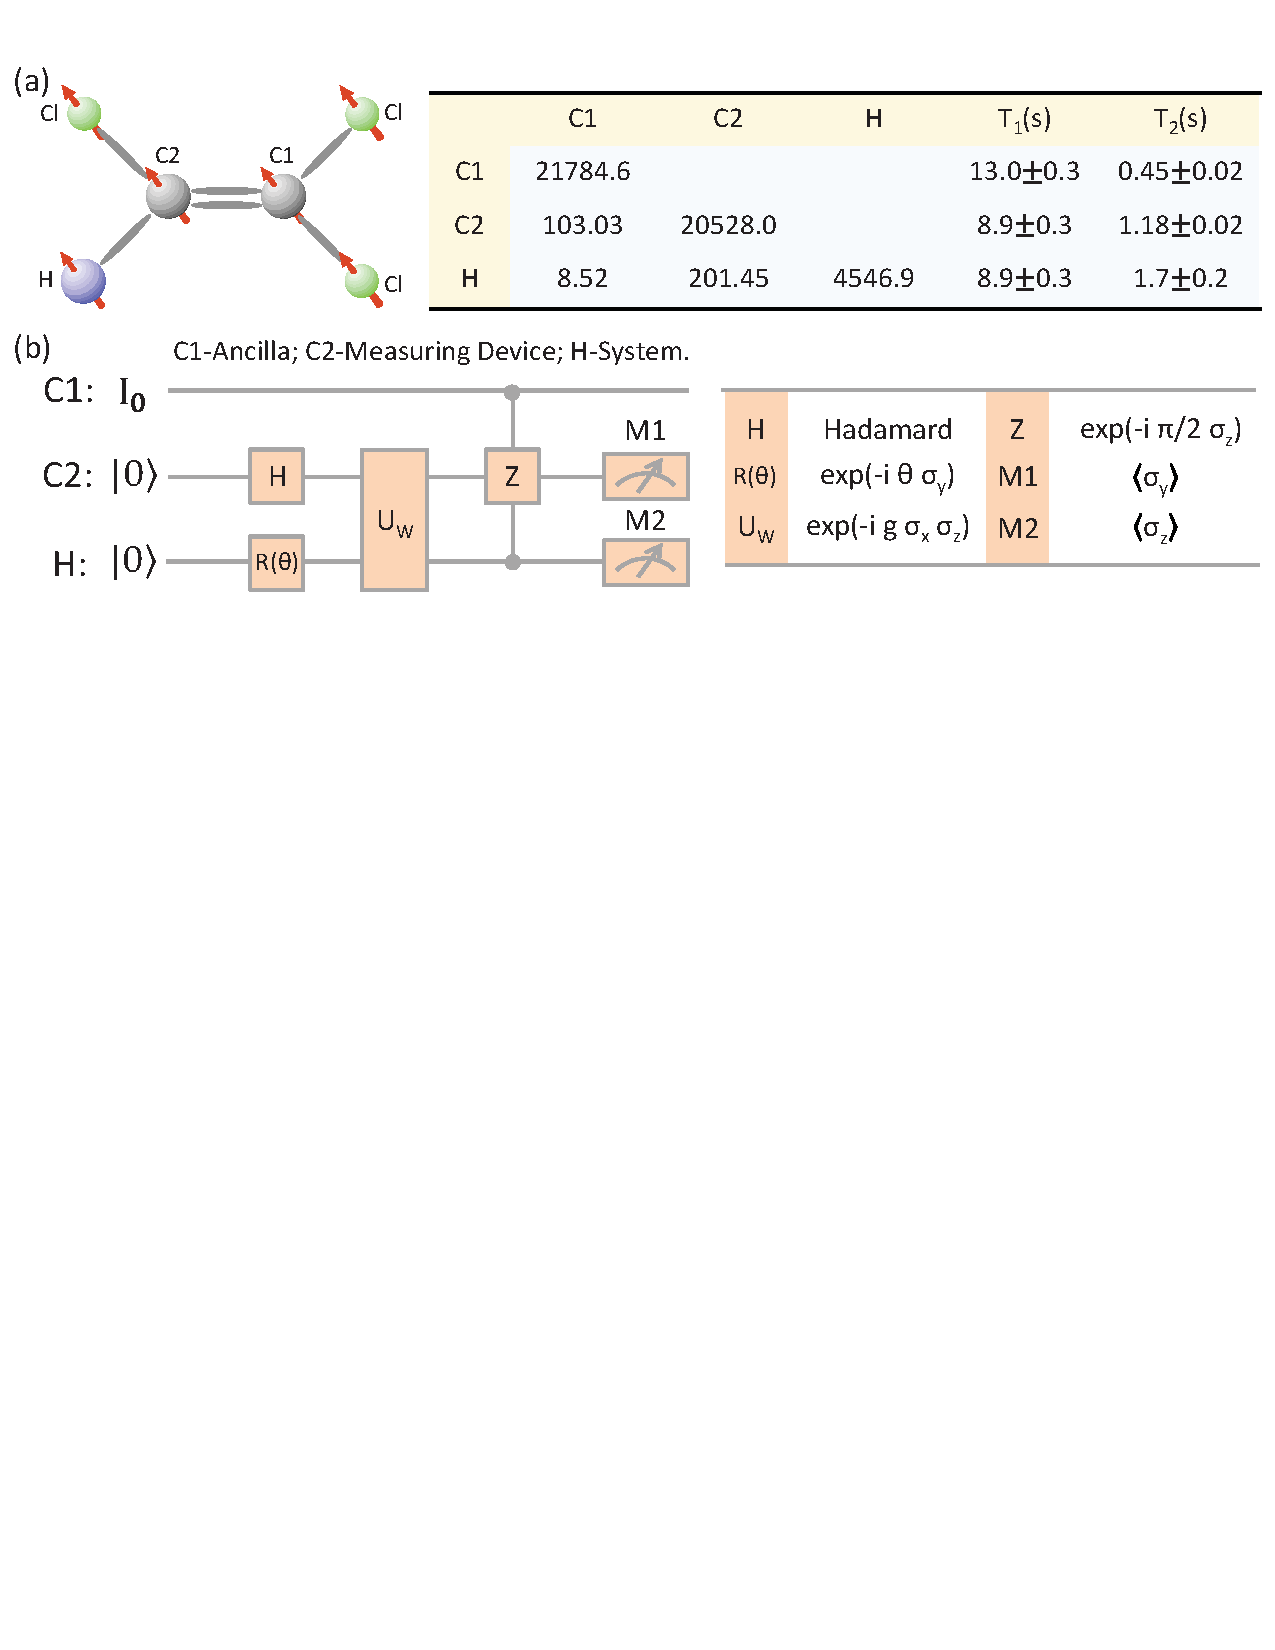
\includegraphics[width=\columnwidth]{molecule.pdf}
\caption{(color online). (a) Molecular structure of trichloroethylene in which the two $^{13}$C and one $^{1}$H spins form a 3-qubit sample, and the system parameters. In the parameter table, the diagonal elements are the chemical shifts (Hz), and the off-diagonal elements are scalar coupling strengths (Hz). The relaxation and dephasing time scales T$_1$ and T$_2$ are also listed in the table. (b) Quantum network to realize the post selected weak measurement in experiment. Here, C1 is used as the ancilla, C2 as the measuring device, and H as the system. }\label{molecule}
\end{figure}

 To realize the post selected weak measurement, we label C1 as the ancilla, C2 as the measuring device, and H as the system displayed in Fig. \ref{molecule}(b). After the labeling, the experiment can be divided into three parts: (A) Initial state preparation. We initialize the ancilla to the identity matrix $I$, the measurement device to $1/\sqrt{2}(|0\rangle+|1\rangle) $, and the system to $cos\theta|0\rangle+sin\theta|1\rangle$. (B) Weak measurement through the interaction between the measuring device and system, denoted by U$_w$ in the network. (C) Post selection of the system in the state $|0\rangle$, with the measurement of $\langle \sigma_y \rangle$ on the measuring device and $\langle \sigma_z \rangle$ on the system subsequently. The experimental details of the three parts above are as follows.

 (A) Initial state preparation.  Starting from the thermal equilibrium state, firstly we excite the ancillar C1 to the transverse field by a $\pi/2$ rotation, followed with a gradient pulse to destroy the coherence. Thus the state of C1 will be maximally mixed state $I$. Secondly we create the pseudopure state (PPS) of the measuring device C2 and system H with deviation $I \otimes | 00 \rangle \langle 00$ using the spatial average technique \cite{spatial}. The spectra of the PPS followed by $\pi/2$ readout pulses are shown in the upper part of Fig. \ref{gweak}(a). The readout pulses are applied on C2 (left figure) and H (right figure), respectively. Two peaks are generated in the PPS spectra because C1 is in the maximally mixed state $I$, and these two peaks are utilized as the benchmark for the following experiments. Thirdly we apply one Hadamard gate on C2 and one $R_y(\theta) = e^{-i\theta\sigma_y}$ rotation on H. Therefore, we have prepared the initial state for the experiment
 \begin{eqnarray}\label{pps}
 \rho_{ini}= &&I\otimes \frac{1}{2} (|0\rangle + |1\rangle) (\langle 0 | + \langle 1 |) \nonumber\\
 &&\otimes  (cos\theta|0\rangle + sin\theta|1\rangle)(cos\theta\langle 0 | + sin\theta\langle 1 |).
 \end{eqnarray}

 (B) Weak measurement. The unitary operater to realize the weak measurement is
 \begin{equation}\label{uw}
U_w=e^{-ig\sigma_x^2 \sigma_z^3}.
 \end{equation}
 Here, without of loss of generality, we have chosen the observable of the measuring device as $\sigma_x$. $U_w$ can be simulated by the interaction term $\sigma_z^2\sigma_z^3$ between C2 and H using the average Hamiltonian theory \cite{ernstbook}. However, since the internal Hamiltonian contains strongly coupling term and the refocusing scheme requires the complicated WAHUHA-4 sequence \cite{wahuha}, we have adopted the gradient ascent pulse engineering (GRAPE) technique \cite{grape1,grape2} to improve the fidelity. We will discuss it in detail later in this letter.

 (C) Post selection. In order to mimic the post selection of $|0\rangle$ on the system spin H in NMR, we need to find one way to implement the controlled resetting noise operation. This can be achieved by introducing an ancilla C1 in the maximally mixed state $I$. The controlled resetting noise operation is thus a controlled-controlled-$\sigma_z$ gate
 \begin{equation}\label{postselection}
I\otimes I \otimes I - |1\rangle \langle 1 | \otimes I \otimes  |1\rangle \langle 1 | + |1\rangle \langle 1 | \otimes |1\rangle \langle 1 | \otimes \sigma_z.
 \end{equation}
 If post selection is successful, the measurement device will point to the weak value. Otherwise the measurement device will become dephased. Finally we measure the expectation value $\langle \sigma_y^2 \rangle$ on C2 and $\langle \sigma_z^3 \rangle$ on H, to calculate the weak value by the expression
 \begin{equation}\label{weakvalue}
\{ \sigma_x \}_w \approx \frac{\langle \sigma_y^2 \rangle}{ g(\langle \sigma_z^3 \rangle+1)}.
 \end{equation}

In the experiment, the $\pi/2$ rotation of H is realized by the hard pulse with a duration of 10 $\mu$s. All the other operations are packed into GRAPE pulses to achieve high-fidelity control. These GRAPE pulses are designed to be robust to the inhomogeneity of the radio frequency, and the imprecisions of the parameters in the Hamiltonian. For the two selective $\pi/2$ excitations on C1 and C2, the GRAPE pulses are generated with the length 1.5 ms, segments 300 and fidelity over 99.95\%. These two pulses are only used for the preparation and observation of PPS. Besides these two GRAPE pulses, the PPS preparation involves another GRAPE pulse of 10 ms and 99.99\% fidelity for the creation of two-body coherence. The upper part of Fig. \ref{gweak}(a) shows the spectra of the PPS both on C2 and H, which are used as the benchmark for the following experiments.

The main body of the network shown in Fig. \ref{molecule}(b), including the initial state preparation, weak measurement and post selection, is calculated by a single GRAPE pulse. Since we have to alter the initial state by $\theta$ and interaction strength $g$ in the experiment, we have used different GRAPE pulses to implement the experiments with different group of parameters. All of the GRAPE pulses have the same length 20 ms, and fidelity over 99.98\%. 

There are two essential advantages in utilizing the GRAPE pulses: reducing the error accumulated by the long pulse sequence if we directly decompose the network, and reducing the error cause by the decoherence. Because the $U_w$ evolution is supposed to be very "weak", the theoretical output signal is quite small. Even, the weak value $\{ \sigma_x \}_w$ is more sensitive to the intensity of the signal, as the small $g$ existing in the denominator (Eq. \ref{weakvalue}) will amplify the errors in the experiment. Therefore, we need to get as accurate coherent control as we can to achieve precise experimental results. The direct decomposition of the original network requires many single rotations, as well as a relatively long evolution time. For example, an efficient way to decompose the controlled-controlled-$\sigma_z$ gate is by six CNOT gates and several one qubit gates \cite{chuangbook}, which requires at least 25 ms regardless of the single qubit gates under the parameters of the Hamiltonian. Therefore, adopting high-fidelity GRAPE pulses will decrease the potential errors extremely in these experiments. The lower part of Fig. \ref{gweak}(a) gives the experimental spectra compared with the simulated one in the case $g=0.05$ and $\theta = 1.4$. The predicted value of $\langle \sigma_y^2 \rangle$ in this case is only 1.67\%. However, since the experimental spectra match very well with the simulated one, we can obtain a good result after extracting the data. See Fig \ref{gweak}(b).

In experiment, firstly we choose three different groups of initial state: $\theta = 1.4$, $\theta = 1.2$, and $\theta =\pi/4$. Then we vary the interaction strength $g$ between the measuring device and system from $g=0.05$ to $g = 0.7$ for a definite $\theta$, and measure $\langle \sigma_y^2 \rangle$ on the measuring device C2 and $\langle \sigma_z^3 \rangle$ on the system H, respectively. The weak value $\{ \sigma_x \}_w$ can be calculated through Eq. \ref{weakvalue}, with the result shown in Fig. \ref{gweak}(b). The error bars are obtained by repeating the experiment for four times and so forth. The large error bars in the weak values when $g$ is small can be contributed to the minor imperfect calibrations of the low experimental signals, and the loss of weak values is mainly caused by the decoherence issue. With the $g$ growing bigger, we can obviously see the experimental data become much better, as the weak measurement is getting closer to strong measurement. 

\begin{figure}[h] \centering
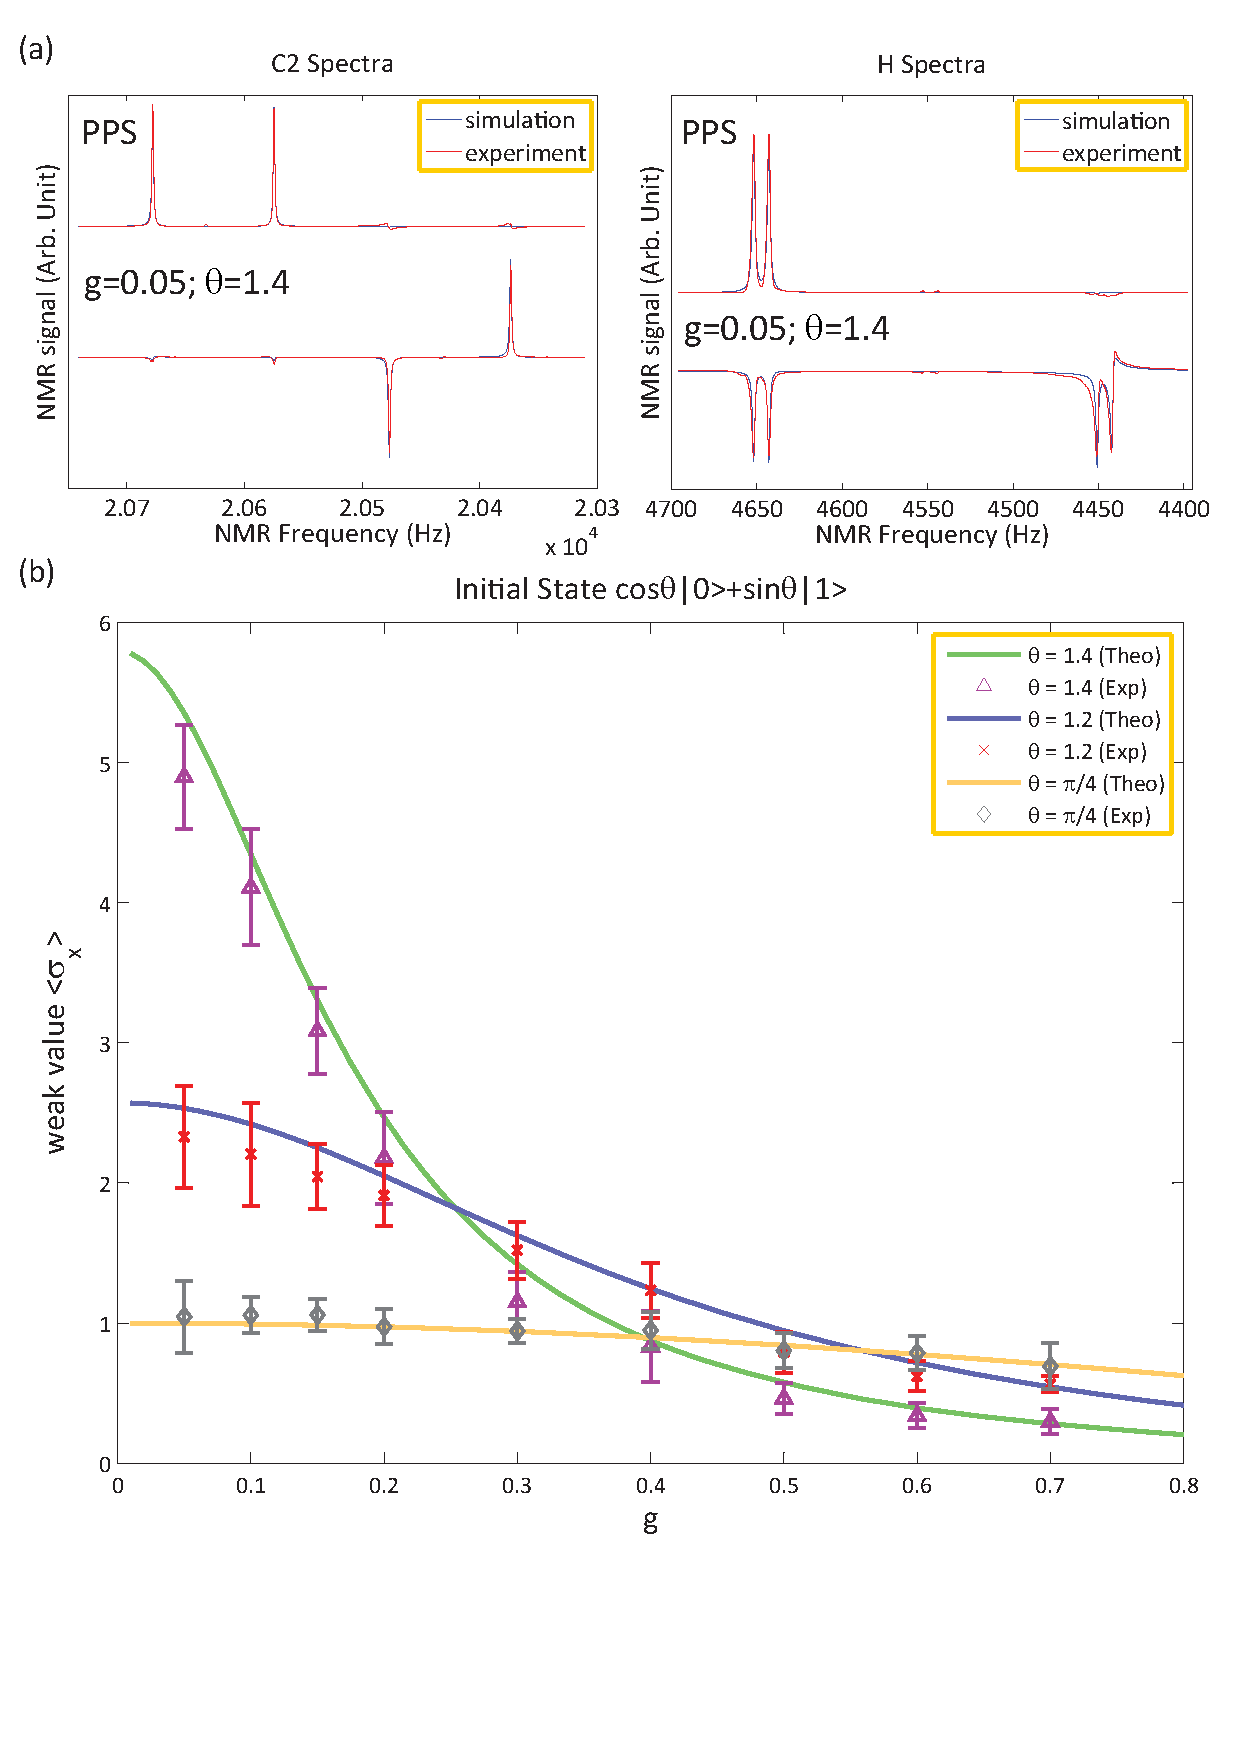
\includegraphics[width=\columnwidth]{gweak.pdf}
\caption{(color online). (a) Spectra for observing $\langle \sigma_y^2 \rangle$ on C2 and $\langle \sigma_z^3 \rangle$ on H in the case $g=0.05$ and $\theta = 1.4$ (lower part), comparing with the PPS spectra (upper part). The blue one is the simulated spectra, while the red one is the experimental spectra. To observe the signal of PPS and $\langle \sigma_z^3 \rangle$ on H, we have applied $\pi/2$ readout pulses after the sequence. To observe the signal of $\langle \sigma_y^2 \rangle$ on C2, we do not need to apply any readout pulses. (b) Experimental result for $g$ $vs$ weak values at three different  initial states. The error bars are plotted by repeating four times experiments.}\label{gweak}
\end{figure}

Secondly we observe the behavior of $\theta$ $vs$ weak by setting $g=0.1$. The theory predicts it should be a perfect $tan\theta$ function when the interaction is infinity weak, $i.e.$, $g$ is infinity close to 0. However, our simulation for $g=0.1$ shows there is singularity when $\theta$ approaches to $\pi/2$ (Fig. \ref{thetaweak}(a)). The explanation is when $\theta \rightarrow \pi/2$, the approximation of the Taylor expansion for small $g$ will be no longer valid. In other words, $g=0.1$ is not small enough to catch up with the effect of $\theta \rightarrow \pi/2$. The experimental data, to some extent, match with the smooth part of the curve. The reason is we cannot measure the extremely low NMR signal due to the signal to noise (SNR) issues for $\theta \rightarrow \pi/2$.

\begin{figure}[h] \centering
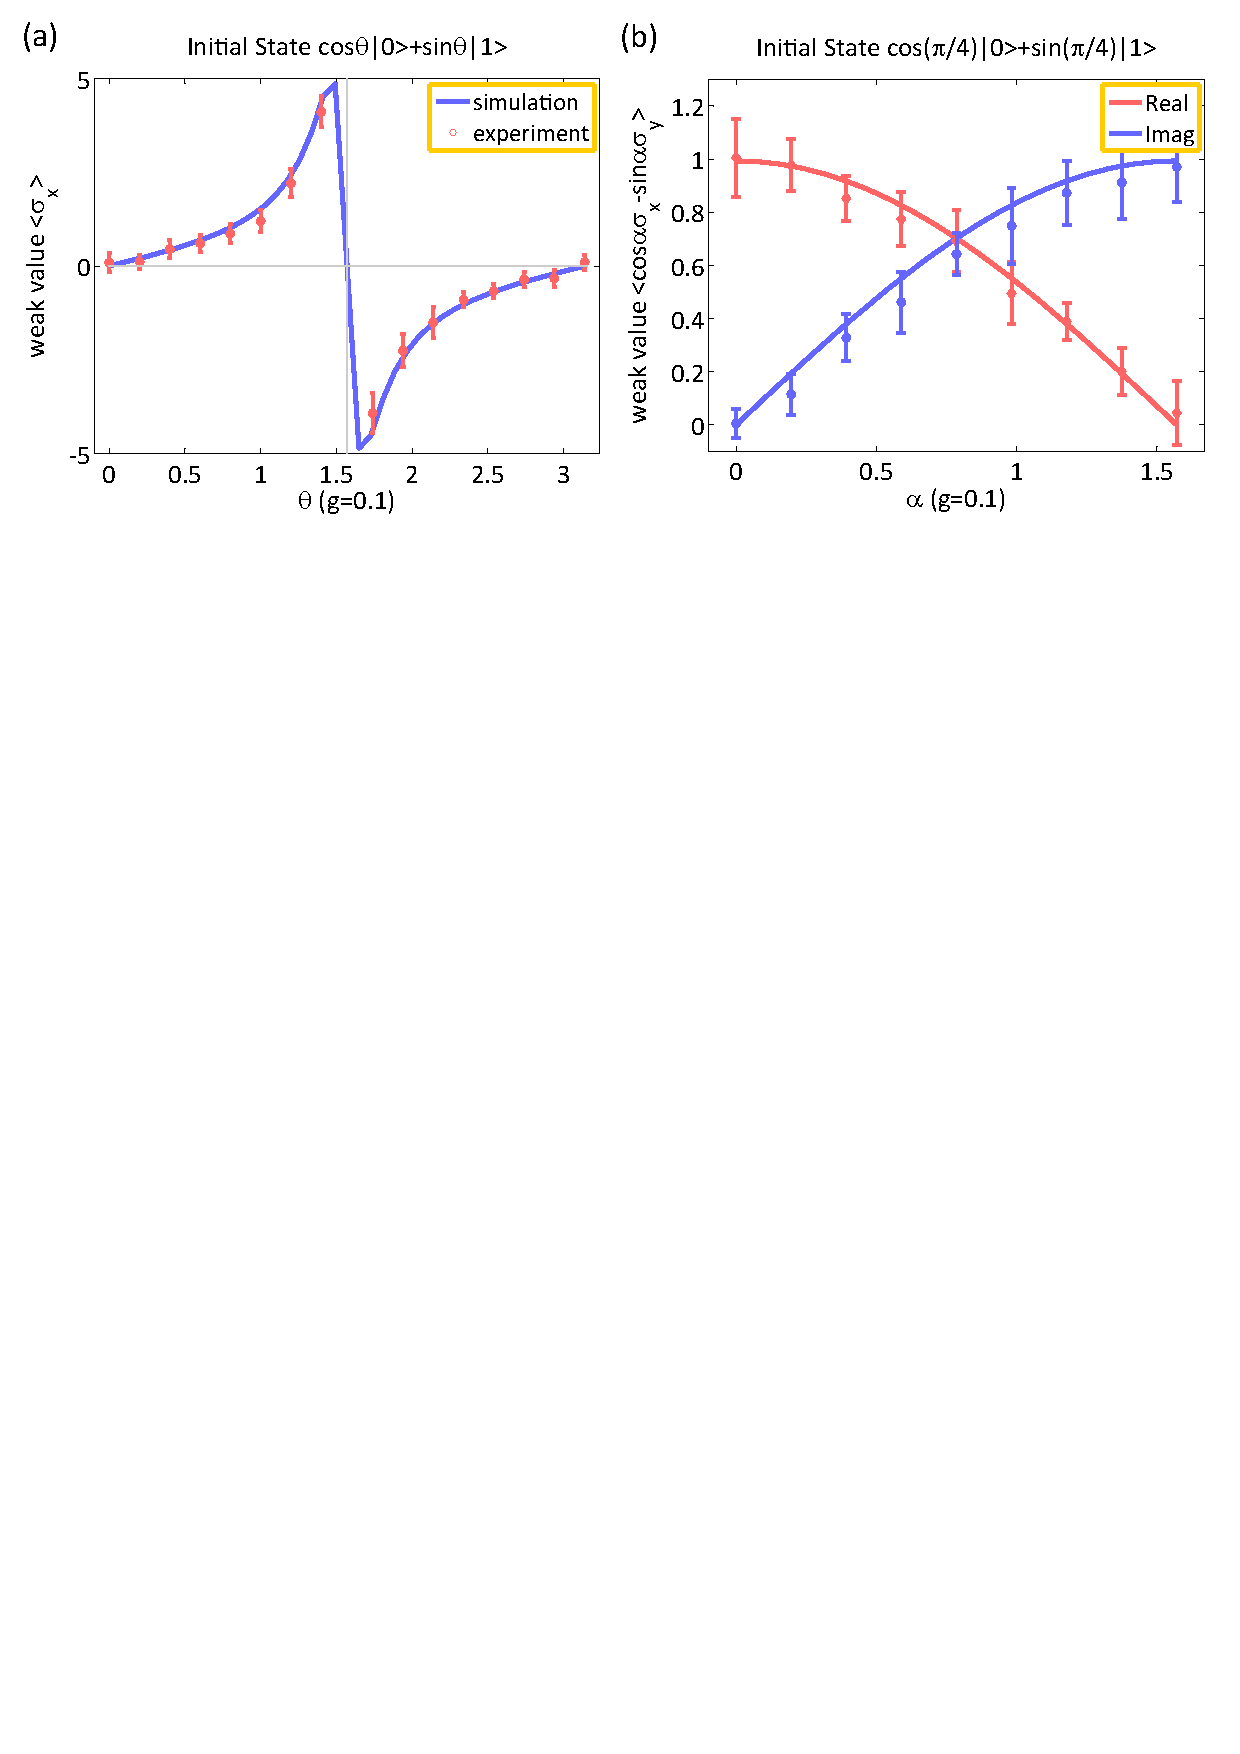
\includegraphics[width=\columnwidth]{thetaweak.pdf}
\caption{(color online). (a) Experimental result of the weak values by changing $\theta$ at $g=0.1$. The simulated (blue) curve is plotted by assuming the weak measurement approximation, and the experimental data are denoted by red circles. (b) Experimental result of measuring both the real and imaginary parts of the weak value at $g=0.1$ and $\theta = \pi/4$. Here we change the observable of the measuring device C2 to $cos\alpha \sigma_x - sin\alpha \sigma_y$.}\label{thetaweak}
\end{figure}

Finally we measure both the real part and imaginary part of the weak value (Fig. \ref{thetaweak}(b)). Here we set $\theta = \pi/4$ and $g=0.1$, and change the observable of the measuring device C2 in the $x-y$ plane by
 \begin{equation}\label{imag}
cos\alpha \sigma_x - sin\alpha \sigma_y.
 \end{equation}
 It is easy to know that the real part of the weak value becomes smaller while the imaginary part of the weak value becomes larger with $\alpha$ varying from 0 to $\pi/2$. To measure the imaginary part, we replace the controlled-controlled-$\sigma_z$ gate in Fig. \ref{molecule}(b) with a controlled-controlled-$\sigma_x$ gate, and measure the expectation value $\sigma_z^2$ on the measuring device C2. The other details of the experiments remain the same. From Fig. \ref{molecule}(b), we can see the alternations of the real part and imaginary part of the weak value along with the parameter $\alpha$.
%\begin{equation}\label{pps}
 %\rho_{I00}=(1-\epsilon)\mathbb{{I}}/8+\epsilon I_0/2 \otimes | 00 \rangle \langle 00 |
 %\end{equation}
 %The thermal equilibrium state in NMR can be written as $\rho_{th} = \sum\nolimits_{i=1}^{3} {\gamma_i \sigma_z^i}$, where $\gamma_i$ is the gyromagnetic ratio for different species of nuclear spins. Typically, $\gamma$_C $=1$ and $\gamma$_H $=4$.





\begin{thebibliography}{28}

\bibitem{nmrreview} L. M. K. Vandersypen and I. L. Chuang, Rev. Mod. Phys. \textbf{76}, 1037 (2004).
\bibitem{spatial} D. G. Cory, A. F. Fahmy, and T. F. Havel, Proc. Natl. Acad. Sci. U.S.A. \textbf{94}, 1634 (1997).
\bibitem{ernstbook} R. R. Ernst, G. Bodenhausen, and A. Wokaun, {\it Principles of Nuclear Magnetic Resonance in One and Two Dimensions}, (Oxford University, Oxford, 1987).
 \bibitem{wahuha} J. S. Waugh, L. M. Huber, and U. Haeberlen, Phys. Rev. Lett. \textbf{20}, 180 (1968).
\bibitem{grape1} N. Khaneja \emph{et al.}, J. Magn. Reson. \textbf{172}, 296 (2005).
\bibitem{grape2} C. A. Ryan, M. Laforest, J. C. Boileau, and R. Laflamme, Phys. Rev. A \textbf{78}, 012328 (2008).
\bibitem{chuangbook} M. A. Nielsen and I. L. Chuang, {\it Quantum Computation and Quantum Information}, (Cambridge University Press, 2000).
\end{thebibliography}











\end{document}
